\documentclass[10pt,a4paper]{article}

\usepackage[utf8]{inputenc}
\usepackage[english]{babel}
\usepackage[english]{isodate}
\usepackage[parfill]{parskip}
\usepackage{courier} % for fixed-width
\usepackage{listings} % for code snippets
\lstset{basicstyle=\ttfamily,
  showstringspaces=false,
  commentstyle=\color{red},
  keywordstyle=\color{black}
}
\usepackage{graphicx}

\begin{document}

\title{LEO2D Manual}
\author{Stephen Carr}
\date{\today}

\maketitle

\pagenumbering{Roman}
\tableofcontents

\newpage
\pagenumbering{arabic}

\section{Introduction}

Locality for electronic obserables in 2D materials (LEO2D) is a code designed to perform parallelized tight-binding calculations in models of twisted 2D heterostructures.

LEO2D is explicitly parallelized with the standard Message Passing Interface (MPI) library, and cannot be run in serial.
The MPI communication is designed in a master-worker queuing system, where a master MPI rank (rank 0) sends out and receives jobs from a series of workers (rank $>$ 0).
The master determines the heterostructure's sparsity pattern, organizes a queue of calculations, and saves results.
Each worker performs a specific realization of the heterostructure hamiltonian, performs relevant electronic structure computations, and then returns results to the master.
For example, when calculating local density of states in finite-systems, the workers handle different local environments.
For periodic systems, the workers perform band-structure sampling by creating the hamiltonian at different k-points.
There is also implicit multi-threading included in the Matrix Kernel Library (MKL), whose routines make up the majority of the work in LEO2D's electronic-structure calculations.

\section{Getting Started}


It is highly recommended that the Intel Matrix Kernal Library (MKL) be used to improve performance on intel hardware.
The MKL includes optimized BLAS and LAPACK routines, which take the majority of wall-time for large tight-binding calculations.


\subsection{Installation}

LEO2D is compiled with the cmake utility.
Make a copy of the \texttt{CMakeLists\_template.txt} named \texttt{CMakeLists.txt} in the same directory.

There are a number of options which can be set to \texttt{ON} or \texttt{OFF} in this file for controlling installation settings:

\begin{itemize}
	\item \textbf{LINK\_FFTW}: Some older compilers do not come with FFTW included by default. This will try to find a FFTW library on the local environment and link it the LEO2D.
	\item \textbf{MKL\_INTEL}: Assumes the MKL library is included in the compiler (works with most modern icc installations).
	\item \textbf{MKL\_GNU}: For use with non-intel compilers (e.g. gcc), will look for the MKL library in the local environment.
	\item \textbf{MKL\_OFF}: Will instead use the open-source C Library Eigen for matrix arithmetic. Eigen has fairly good matrix-vector multiplication, but its diagonalization is much slower than the MKL LAPACK routines.
\end{itemize}

When finished, the executable \texttt{LEO2D} should be available in the \texttt{app/} directory, and a partner library \texttt{libleo2d.a} will be in the \texttt{lib/} directory.

\subsection{Running Examples}

Once compiled, try running LEO2D on any of examples provided in the \texttt{examples} directory.
For example, to run a supercell band-structure calculation for twisted bilayer graphene, go to the \texttt{example/tblg\_sc} directory and call LEO2D like so:

\begin{lstlisting}
mpirun -n 2 ../../app/LEO2D tblg_sc_hstruct.in
\end{lstlisting}

Here we are calling a 2-core instance of LEO2D using the settings in \texttt{tblg\_sc\_hstruct.in}.
The same can be done for any of the other examples.
Note that the \texttt{examples/old/} directory is no longer maintained.

\begin{figure}
  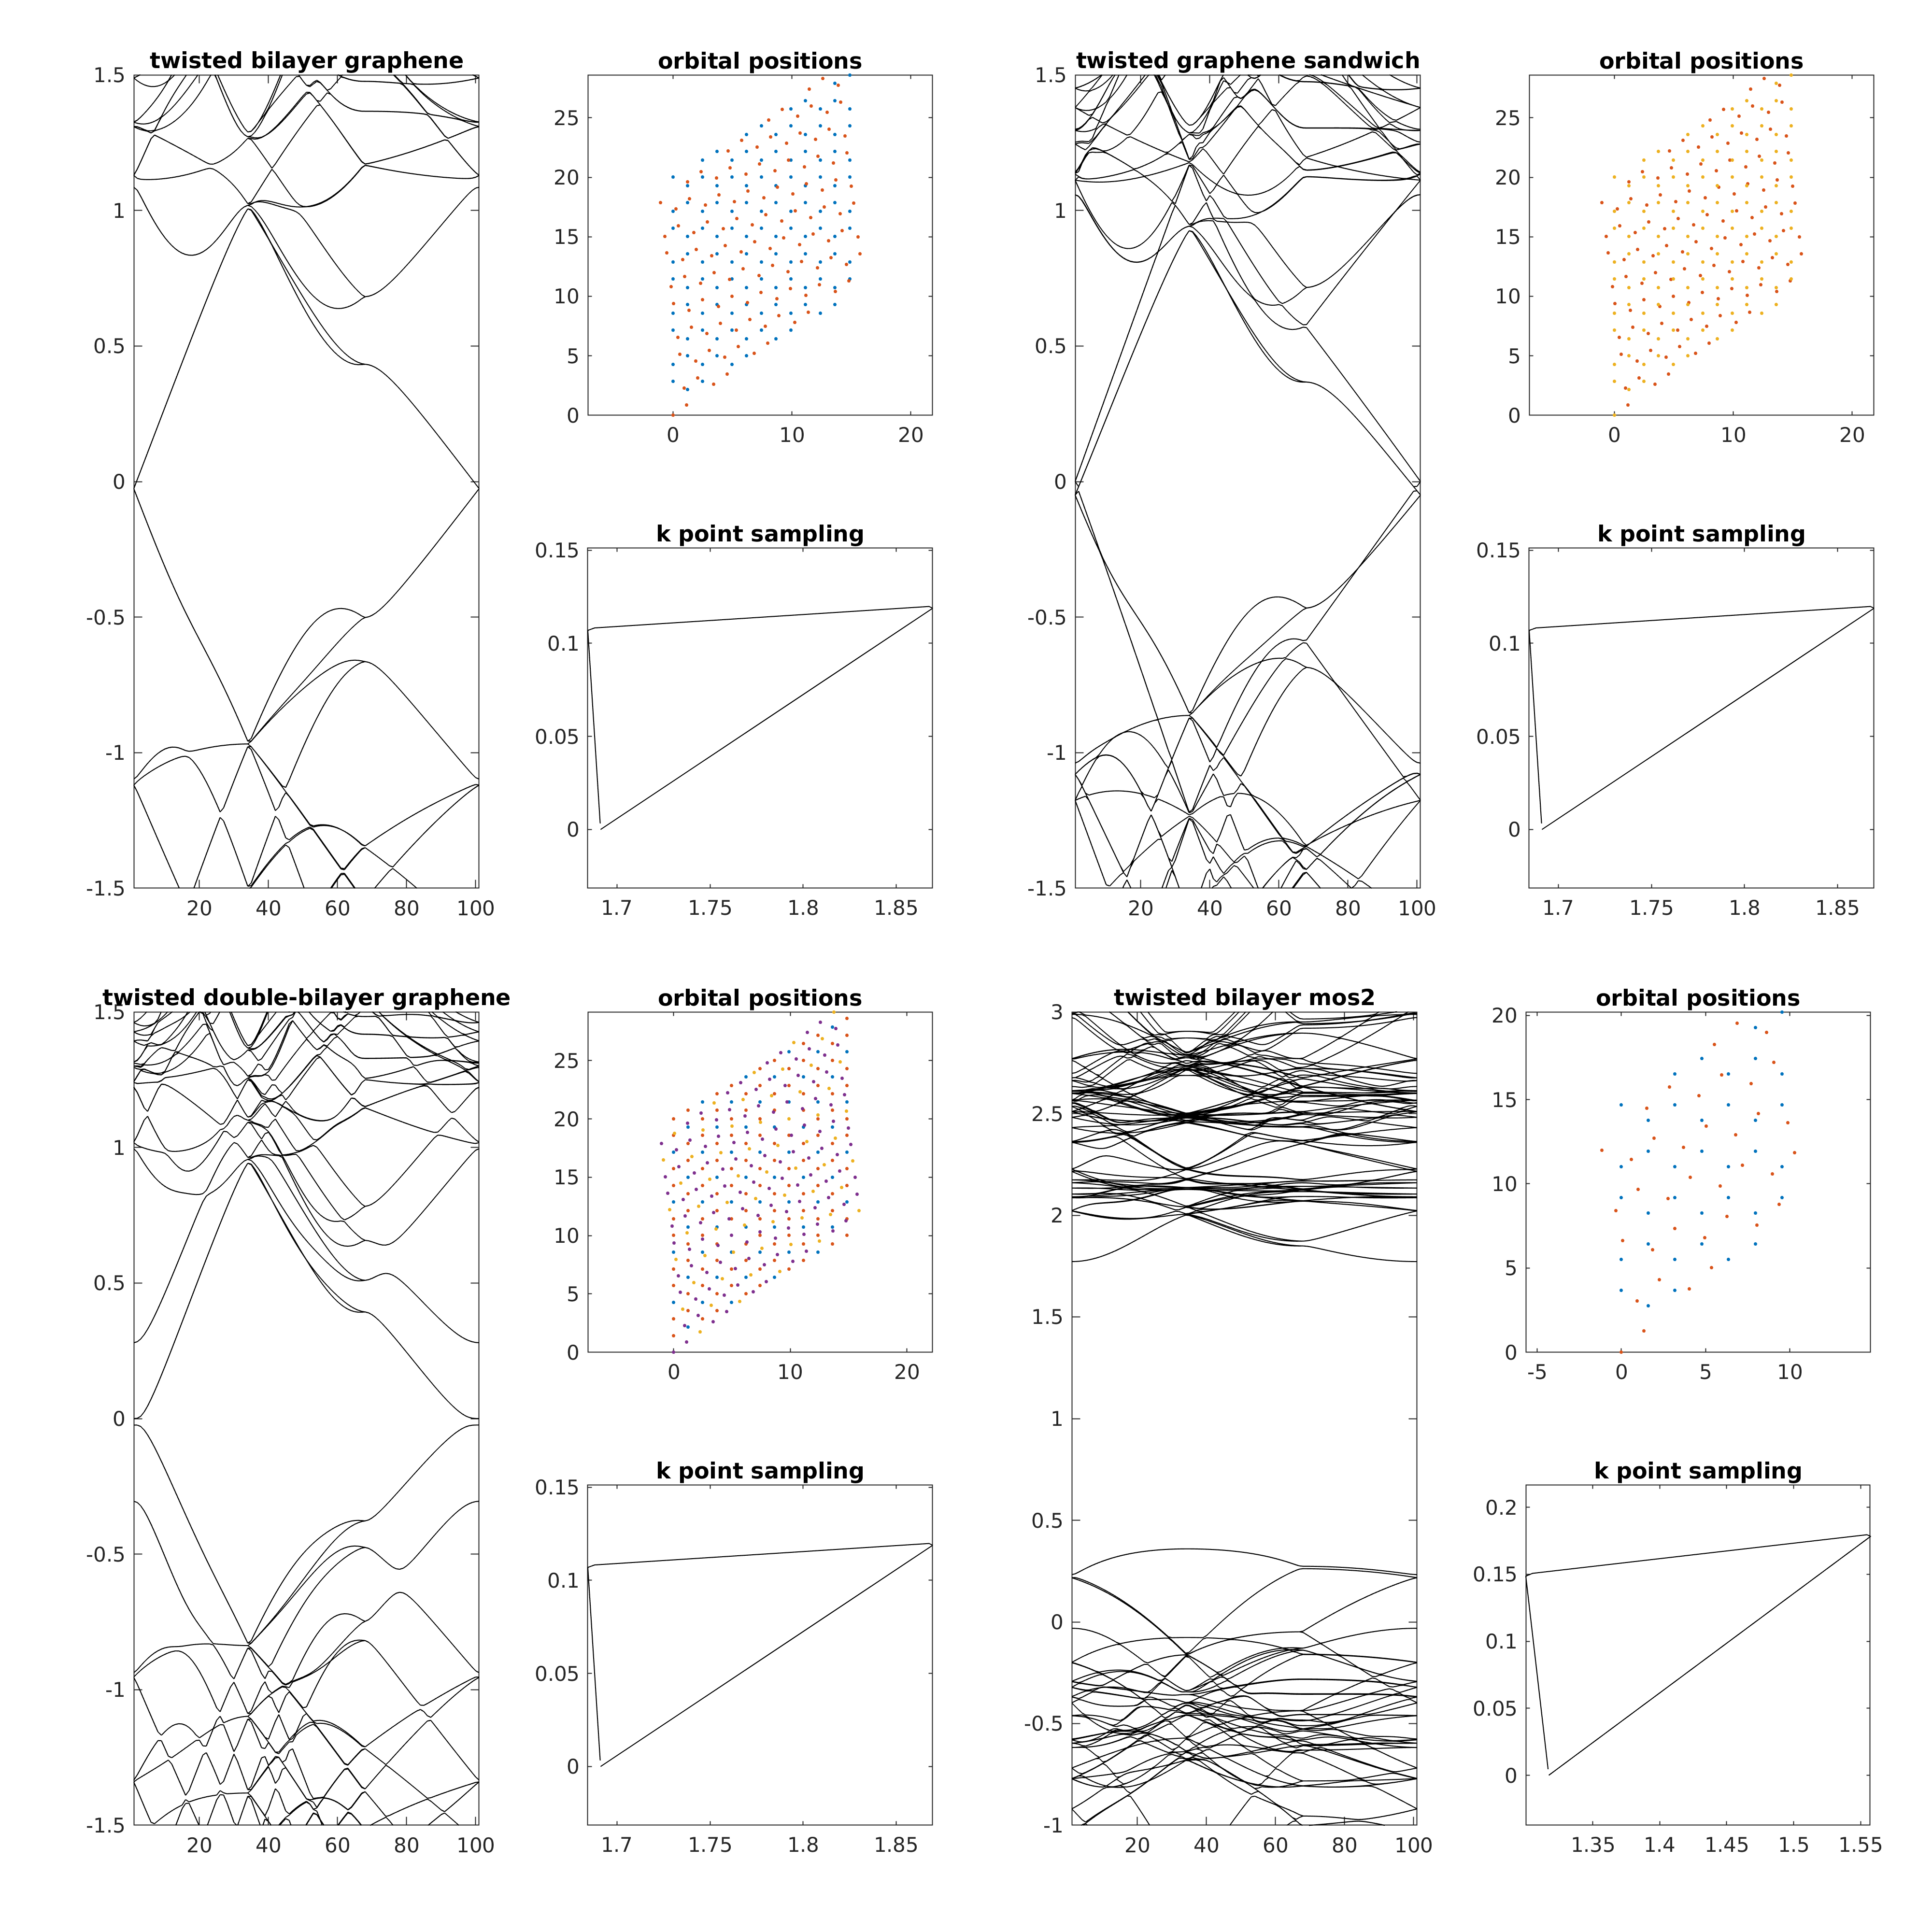
\includegraphics[width=\textwidth]{supercell_examples.png}
  \caption{
  Supercell band-structure examples.
  }
  \label{fig:tblg_sc}
\end{figure}

There are four twisted supercell examples: bilayer graphene (\texttt{tblg\_sc}), graphene sandwich (\texttt{tswg\_sc}), double-bilayer graphene (\texttt{tdbg\_sc}), and bilayer MoS$_2$ (\texttt{tbmos2\_sc}).
There is also and example of a density of states calculation for a twisted finite flake (\texttt{tblg\_flake}) and for a bandstructure comparison for monolayer graphene with and without a uniform strain (\texttt{mlg\_strain}).



\subsection{Common Errors}

\section{Parameters}

\section{Code Overview}

\end{document}